\documentclass[10pt,UTF8]{ctexart}
\usepackage{amsmath}
\usepackage{graphicx}
\usepackage{hyperref}
\usepackage{underscore}
\hypersetup{ colorlinks=true, linkcolor=blue, filecolor=gray, urlcolor=blue, citecolor=blue, }
\title{表达式}
\author{ZhangXu}
\begin{document}
\maketitle
\part{Expressions}
本章解释了Python中表达式元素的含义。\\
\indent 语法注释:在本章和后续章节中,扩展的BNF表示法将用于描述语法,而不是词法分析。当(一种替代)语法规则具有表单:\\
\textbf{name} ::= othername\\
\indent 并且没有给出语义,这种形式的name的语义与othername的语义相同。
\section{算术转换(Arithmetic conversions)}
当下面的算术运算符的描述使用短语“数字参数转换为公共类型”时,这意味着内置类型的运算符实现的工作方式如下:
\begin{itemize}
\item 如果任一参数是复数,则另一个参数转换为复数;
\item 否则,如果任一参数是浮点数,则另一个转换为浮点数;
\item 否则,两者必须是整数,不需要转换。
\end{itemize}
某些附加规则适用于某些运算符(例如,字符串作为'\%'运算符的左参数)。扩展必须定义自己的转换行为。
\section{原子}
原子是\textbf{表达式中最基本的元素}。最简单的原子是标识符(identifiers )或文字(literals)。括在括号,括号或大括号中的表单也在语法上被分类为原子。原子的语法是:\\
\textbf{atom} ::= identifier | literal | enclosure\\
\textbf{enclosure} ::= parenth_form | list_display | dict_display | set_display | generator_expression | yield_atom
\subsection{标识符(名称)Identifiers(Name)}
作为原子出现的标识符是名称。请参阅词法定义的标识符和关键字部分(\href{https://docs.python.org/3/reference/lexical_analysis.html#identifiers}{Identifiers and keywords})以及命名和绑定文档的命名和绑定部分。\\
\indent 当名称绑定到对象时,对atom的计算会产生该对象。如果未绑定名称,则尝试对其进行评估会引发NameError异常。
\paragraph{私人名称(Private name mangling):}如果在类定义中以文本方式出现的标识符以两个或多个下划线字符开头,并且不以两个或多个下划线结尾,则将其视为该类的私有名称(private name)。在为其生成代码之前,将私有名称转换为更长的形式。\textbf{转换将在名称前面插入类名,删除前导下划线并插入单个下划线。}例如,名为Ham的类中出现的标识符__spam将转换为_Ham__spam。此转换独立于使用标识符的语法上下文。如果转换后的名称非常长(超过255个字符),则可能会发生实现定义的截断。如果类名仅由下划线组成,则不进行转换。
\section{Literals字面值}
Python支持字符串和字节文字以及各种数字文字:\\
\textbf{literal} ::= stringliteral | bytesliteral | interger | floatnumber | imagnumber\\
对文字的计算产生具有给定值的给定类型的对象(字符串,字节,整数,浮点数,复数)。在浮点和虚(复)字面的情况下,该值可以近似。有关详细信息,请参阅\href{https://docs.python.org/3/reference/lexical_analysis.html#literals}{Literal}部分。\\
\indent 所有文字都对应于不可变数据类型,因此对象的标识不如其值重要。对具有相同值的文字的多次计算(在程序文本中出现相同或不同的出现)可以获得具有相同值的相同对象或不同对象。
\subsection{Parenthesized forms}
A parenthesized form是括在括号中的可选表达式列表:\\
\textbf{parenth_form} ::= "(" [starred_expression] ")"\\
\indent 带括号的表达式列表产生表达式列表产生的任何内容:如果列表包含至少一个逗号,则它产生一个元组;否则,它会产生构成表达式列表的单个表达式。\\
\indent 一对空括号产生一个空元组对象。由于元组是不可变的,因此适用字面值规则(即,两次出现的空元组可能会或可能不会产生相同的对象)。\\
\indent 请注意,元组不是由括号组成,而是使用逗号运算符。唯一的例外是空元组,需要括号 - 在表达式中允许不带括号的“无”会导致含糊不清并允许常见错别字传递未被捕获。
\subsection{Display for 列表,集合和词典}
为了构造一个列表,一个集合或一个字典,Python提供了一种称为""的特殊语法,每种语法都有两种形式:
\begin{itemize}
\item 容器内容是明确列出的,或者
\item 它们是通过一组循环和过滤指令计算出来的,称为$\mathit{comprehension}$。
\end{itemize}
Common syntax elements for $\mathit{comprehension}$ are:\\
\textbf{comprehension} ::= expression comp_for
comp_for ::= ["async"] "for" target_list "in" or_test [comp_iter]
comp_iter ::= comp_for | comp_if
comp_if ::= "if" expression_nocond [comp_iter]\\
\indent comprehension包括单个表达式,后跟至少一个for子句和零个或多个for或if子句。在这种情况下,新容器的元素是通过将每个for或if子句从左到右嵌套,并且每次到达最内部块时计算表达式以产生元素而生成的元素。\\
\indent 但是,除了最左边的for子句中的iterable表达式之外,comprehension还在一个单独的隐式嵌套作用域中执行。这可确保分配给目标列表中的名称不会"泄漏"到封闭范围中。\\
\indent 最左边的for子句中的可迭代表达式直接在封闭范围内计算,然后作为参数传递给隐含嵌套的范围。对于子句的后续条件和最左侧for子句中的任何过滤条件都不能在封闭范围内进行计算,因为它们可能取决于从最左边的可迭代获得的值。 For example: $[x*y for x in range(10) for y in range(x, x+10)]$。\\
\indent 为了确保comprehension总是产生适当类型的容器,在隐式嵌套范围内禁止表达式的yield 和 yield form(在Python 3.7中,这样的表达式在编译时发出DeprecationWarning,在Python 3.8+中它们将发出SyntaxError)\\
\indent 从Python 3.6开始,在async def函数中,可以使用async for子句迭代异步​​迭代器。async def函数中的理解可以包括前导表达式后面的for或async for子句,可以包含附加for或async for子句,也可以使用await表达式。如果comprehension包含async for 短句或await表达式,则称为异步理解(asynchronous comprehension)。异步理解可以暂停其出现的协程函数的执行。另见PEP 530。\\
\indent 从版本3.7开始不推荐使用:在隐式嵌套范围中弃用的yield和yield from。
\subsection{列表显示List displays}
列表显示是用方括号括起来的可能为空的一系列表达式:\\
\textbf{list_display} ::= "[" [starred_list | comrehension] "]"\\
\indent 列表显示产生一个新的列表对象,内容由表达式列表或comprehension指定。当提供以逗号分隔的表达式列表时,其元素将从左到右进行计算,并按该顺序放入列表对象中。当提供comprehension时,列表由comprehension产生的元素构成。
\subsection{集合显式set displays}
集合显示用花括号表示,并且由于缺少由冒号分隔的键和值而与字典显示区分开来:
\textbf{set_display} ::= "{" (starred_list | comprehension) "}"
集合显示产生新的可变集合对象,内容由表达式序列或comprehension指定。当提供以逗号分隔的表达式列表时,将从左到右计算其元素并将其添加到set对象。当提供comprehension时,该集合由comprehension产生的元素构成。\\
\indent 无法用{}构造空集;这个文字构造了一个空字典。
\subsection{字典显示}
字典显示是用花括号括起来的可能为空的一系列键/数据对:\\
dict_display ::= "{" [key_datum_list | dict_comprehension] "}"\\
key_datum_list ::=  key_datum ("," key_datum)* [","]\\
key_datum ::=  expression ":" expression | "**" or_expr\\
dict_comprehension ::=  expression ":" expression comp_for\\
\indent 字典显示产生新的字典对象。\\
\indent 如果给出了以逗号分隔的 key/datum对序列,则从左到右对它们进行求值以定义字典的条目:每个键对象用作字典中的键以存储相应的数据。这意味着您可以在 key/datum列表中多次指定相同的键,并且该键的最终字典值将是给定的最后一个键。\\
\indent 双星号**表示字典解包(dictionary unpacking)。它的操作数必须是映射。每个映射项都添加到新字典中。后面的值替换先前由key/datum对和早期字典解包设置的值。\\
\indent 与list和set comprehensions相反,dict comprehension需要两个用冒号分隔的表达式,后跟通常的“for”和“if”子句。运行理解时,生成的键和值元素将按照生成的顺序插入到新字典中。
\subsection{生成器表达式}
生成器表达式是括号中的紧凑生成符:\\
\textbf{generator_expression} ::= "(" expression comp_for ")"\\
\indent 生成器表达式生成一个新的生成器对象。它的语法与comprehension相同,只是它括在括号中而不是括号或花括号中。\\
\indent 当为生成器对象调用__next __()方法时,与生成器表达式中使用的变量会被惰性计算(与普通生成器一样)。但是,会立即计算最左侧for子句中的可迭代表达式,以便在定义生成器表达式的位置(而不是在检索第一个值的位置)发出由它生成的错误。对于子句的后续条件和最左侧for子句中的任何过滤条件都不能在封闭范围内进行求值,因为它们可能取决于从最左边的可迭代获得的值。 For example: (x*y for x in range(10) for y in range(x, x+10)).\\
\indent 对于只有一个参数的调用,可以省略括号。请参阅\href{https://docs.python.org/3/reference/expressions.html#calls}{Call}部分了解详情。\\
\indent 为了避免干扰生成器表达式本身的预期操作,在隐式定义的生成器中禁止表达式的yield和yield from(在Python 3.7中,这样的表达式在编译时发出DeprecationWarning,在Python 3.8+中它们将发出SyntaxError)。\\
\indent 如果生成器表达式包含async for或await表达式,则称为异步生成器表达式。异步生成器表达式返回一个新的异步生成器对象,它是一个异步迭代器(请参阅\href{https://docs.python.org/3/reference/datamodel.html#async-iterators}{异步迭代器(Asynchronous Iterators)})
\subsection{Yield expressions}
yield_atom =::= "(" yield_expression ")"\\
yield_expression ::=  "yield" [expression_list | "from" expression]\\
\indent yield表达式在定义生成器函数或异步生成器函数时使用,因此只能在函数定义的主体中使用。在函数体中使用yield表达式会导致该函数成为生成器,并且在异步def函数体中使用它会导致该协同函数成为异步生成器。例如:\\
def gen():yield 123  \# defines a generator function\\
async def agen(): yield 123 \# defines an asynchronos generator function\\
\indent 由于它们对包含范围的副作用,yield表达式不允许作为用于实现comprehensions 和generator expressions的隐式定义范围的一部分(在Python 3.7中,此类表达式在编译时发出DeprecationWarning,在Python 3.8+中它们将发出SyntaxError)。\\
\indent 下面描述了生成器函数(generator functions),而asynchronous generator functions异步生成器函数在\href{https://docs.python.org/3/reference/expressions.html#asynchronous-generator-functions}{Asynchronous generator functions}.部分中单独描述。\\
\indent 当调用生成器函数时,它返回一个称为生成器的迭代器。然后该生成器控制生成器函数的执行。当调用其中一个生成器的方法时,执行开始。那时,执行进入第一个yield表达式,再次暂停,将expression_list的值返回给生成器的调用者。通过挂起,我们的意思是保留所有本地状态,包括局部变量的当前绑定,指令指针,内部计算堆栈以及任何异常处理的状态。当通过调用生成器的一个方法恢复执行时,该函数可以完全像yield表达式只是另一个外部调用一样。恢复后yield表达式的值取决于恢复执行的方法。如果使用__next __()(通常通过for或next()内置),则结果为None。否则,如果使用send(),则结果将是传递给该方法的值。\\
\indent 所有这些使得生成器功能与协同程序非常相似;它们产生多次,它们有多个入口点并且它们的执行可以被暂停。唯一的区别是生成器函数无法控制执行后应该继续执行的位置;控制器总是转移到生成器的调用者。\\
\indent 在try构造中的任何位置都允许yield表达式。如果生成器在最终确定之前没有恢复(通过达到零引用计数或通过垃圾收集),将调用generator-iterator的close()方法,允许执行任何挂起的finally子句。\\
\indent 当使用yield from <expr>时,它将提供的表达式视为子实例。该子转换器生成的所有值都直接传递给当前生成器方法的调用者。使用send()传入的任何值以及使用throw()传递的任何异常都会传递给底层迭代器(如果它具有适当的方法)。如果不是这种情况,那么send()将引发AttributeError或TypeError,而throw()将立即引发传入的异常。底层迭代器完成后,引发的StopIteration实例的value属性将成为yield表达式的值。它可以在 raising StopIteration时显式设置,也可以在子迭代器是生成器时自动设置(通过从子生成器返回值)。\\
\indent 当yield表达式是赋值语句右侧的唯一表达式时,可省略括号。
\begin{itemize}
\item PEP 255 - Simple Generators
\item PEP 342 - Coroutines via Enhanced Generators
\item PEP 380 - Syntax for Delegating to a Subgenerator
\item PEP 525 - Asynchronous Generators
\end{itemize}
\subsubsection{Generator-iterator方法}
本小节描述了生成器迭代器的方法。它们可用于控制生成器功能的执行。请注意,在生成器已在执行时调用以下任何生成器方法会引发ValueError异常。
\paragraph{generator.__next__()}
开始执行生成器函数或在最后执行的yield表达式中恢复它。当使用__next __()方法恢复生成器函数时,当前yield表达式始终求值为None。然后执行继续到下一个yield表达式,再次暂停生成器,并将expression_list的值返回给__next __()的调用者。如果生成器退出而不产生另一个值,则引发StopIteration异常。\\
\indent 这种方法通常是隐式调用的,例如,通过for循环,或通过内置的next()函数。
\paragraph{generator.send(value)}
恢复执行并将值“发送”到生成器函数中。 value参数成为当前yield表达式的结果。send()方法返回生成器产生的下一个值,如果生成器退出而不产生另一个值,则引发StopIteration。当调用send()来启动生成器时,必须使用None作为参数调用它,因为没有可以接收该值的yield表达式。
\paragraph{generator.throw(type[,value[,traceback]])}
在生成器暂停的位置引发类型type的异常,并返回由生成器函数生成的下一个值。如果生成器退出而不产生另一个值,则引发StopIteration异常。如果生成器函数没有捕获传入的异常,或者引发另一个异常,那么该异常会传播给调用者。
\paragraph{generator.close()}
在生成器功能暂停的位置引发GeneratorExit。如果生成器函数正常退出,然后已经关闭,或者引发GeneratorExit(通过不捕获异常),则关闭返回其调用者。如果生成器产生一个值,则引发RuntimeError。如果生成器引发任何其他异常,它将传播给调用者。如果由于异常或正常退出,生成器已经退出,则close()不执行任何操作。\\
\indent 有关使用yield from的示例,请参阅\href{https://docs.python.org/3/whatsnew/3.3.html#pep-380}{PEP 380:在“Python中的新功能”}中委派给子生成器的语法。
\subsubsection{Asynchronous generator functions}
在使用async def定义的函数或方法中存在yield表达式进一步将该函数定义为异步生成器函数。\\
\indent 当调用异步生成器函数时,它返回一个称为异步生成器对象的异步迭代器。然后该对象控制生成器函数的执行。异步生成器对象通常用在协程函数中的async for语句中,类似于如何在for语句中使用生成器对象。\\
\indent 调用其中一个异步生成器的方法会返回一个等待对象,并在等待该对象时开始执行。那时,执行继续执行第一个yield表达式,再次暂停,将expression_list的值返回到等待协同程序。与生成器一样,暂停意味着保留所有本地状态,包括局部变量的当前绑定,指令指针,内部计算堆栈以及任何异常处理的状态。当等待异步生成器的方法返回的下一个对象恢复执行时,该函数可以像yield表达式只是另一个外部调用一样继续。恢复后yield表达式的值取决于恢复执行的方法。如果使用__anext __(),则结果为None。否则,如果使用asend(),则结果将是传递给该方法的值。\\
\indent 在异步生成器函数中,yield构造中允许使用yield表达式。但是,如果异步生成器在最终确定之前未恢复(通过达到零引用计数或通过垃圾回收),则try结构中的yield表达式可能导致无法执行挂起的finally子句。在这种情况下,运行异步生成器的事件循环或调度程序负责调用异步生成器 - 迭代器的aclose()方法并运行生成的协程对象,从而允许执行任何挂起的finally子句。\\
\indent 为了完成最终化,一个事件循环应该定义一个终结器函数,它接受一个异步生成器 - 迭代器,并且可能调用aclose()并执行协程。可以通过调用sys.set_asyncgen_hooks()来注册此终结器。首次迭代时,异步生成器迭代器将存储在完成时调用的已注册终结器。有关终结器方法的参考示例,请参阅\href{https://github.com/python/cpython/blob/3.7/Lib/asyncio/base_events.py}{Lib/asyncio/ base_events.py}中asyncio.Loop.shutdown_asyncgens的实现。\\
\indent 当在异步生成器函数中使用yield from <expr>时,其是语法错误。
\subsubsection{异步生成器 - 迭代器方法(Asynchronous generator-iterator methods)}
本小节描述了异步生成器迭代器的方法,它们用于控制生成器函数的执行
\paragraph{coroutine agen.__anext__()}返回一个awaitable,当运行开始执行异步生成器或在最后执行的yield表达式恢复它时。当使用__anext __()方法恢复异步生成器函数时,当前yield表达式总是在返回的awaitable中计算为None,运行时将继续执行下一个yield表达式。yield表达式的expression_list的值是完成协程引发的StopIteration异常的值。如果异步生成器退出而不产生另一个值,则等待引发StopAsyncIteration异常,表示异步迭代已完成。\\
\indent 此方法通常由异步for循环隐式调用。
\paragraph{coroutine agen.asend(value)}返回一个awaitable ,当运行时恢复异步生成器的执行。与生成器的send()方法一样,这将“发送”一个值到异步生成器函数中,value参数成为当前yield表达式的结果。asend()方法返回的等待将返回生成器产生的下一个值作为引发的StopIteration的值,或者如果异步生成器退出而不产生另一个值,则引发StopAsyncIteration。当调用asend()来启动异步生成器时,必须使用None作为参数调用它,因为没有可以接收该值的yield表达式。
\paragraph{coroutine agen.athrow(type[,value[,traceback]]}
返回一个awaitable,它在异步生成器暂停时引发类型类型的异常,并返回生成器函数产生的下一个值作为引发的StopIteration异常的值。如果异步生成器退出而不产生另一个值,则等待引发StopAsyncIteration异常。如果生成器函数没有捕获传入的异常,或者引发另一个异常,那么当等待运行时,该异常会传播给等待的调用者。
\paragraph{coroutine agen.aclose()}
返回一个awaitable,当运行时会将GeneratorExit抛出到异步生成器函数暂停的位置。如果异步生成器函数正常退出,然后已经关闭,或者引发GeneratorExit(通过不捕获异常),则返回的等待将引发StopIteration异常。后续调用异步生成器返回的任何进一步的等待都会引发StopAsyncIteration异常。如果异步生成器产生一个值,则等待引发RuntimeError。如果异步生成器引发任何其他异常,它将传播给等待的调用者。如果异步生成器由于异常或正常退出而已经退出,那么对aclose()的进一步调用将返回一个不执行任何操作的等待。
\section{Primaries原语}
Primaries代表语言最紧密的操作。他们的语法是:\\
primary ::= atom | attributeref | subscription | slicing | call
\subsection{属性引用}
属性引用是主要的,后跟句点和名称:\\
attributeref ::=  primary "." identifier\\
\indent primary必须求值为支持属性引用的类型的对象,大多数对象都这样做。然后要求该对象生成名称为标识符的属性。可以通过重写__getattr__()方法来自定义此产生方式。
如果此属性不可用,则引发异常AttributeError。否则,生成的对象的类型和值由对象确定。对同一属性引用的多次计算可能产生不同的对象。
\subsection{Subscriptions}
Subscriptions选择序列(字符串,元组或列表)或映射(字典)对象的项:\\
subscription ::=  primary "[" expression_list "]"\\
\indent primary必须计算支持subscription的对象(例如列表或字典)。用户定义的对象可以通过定义__getitem__()方法来支持订阅。\\
\indent 对于内置对象,有两种类型的对象支持subscription:\\
\indent 如果primary是映射,则表达式列表必须求值为其值为映射的键之一的对象,并且 subscription 选择映射中与该键对应的值。 (表达式列表是一个元组,除非它只有一个项目。)\\
\indent 如果primary是序列,则表达式列表必须求值为整数或切片(如下一节中所述)。\\
\indent 形式语法对序列中的负索引没有特殊规定;但是,内置序列都提供__getitem __()方法,通过将序列的长度添加到索引来解释负索引(以便x [-1]选择x的最后一项)。结果值必须是小于序列中项目数的非负整数,并且subscription选择索引为该值的项目(从零开始计数)。由于对负索引和切片的支持发生在对象的__getitem __()方法中,因此重写此方法的子类将需要显式添加该支持。\\
\indent 字符串的项目是字符。字符不是单独的数据类型,而是一个恰好一个字符的字符串。
\subsection{切片Slicings}
切片选择序列对象中的一系列项(例如,字符串,元组或列表)。切片可以用作赋值或del语句中的表达式或目标。切片的语法:\\
slicing      ::=  primary "[" slice_list "]"\\
slice_list   ::=  slice_item ("," slice_item)* [","]\\
slice_item   ::=  expression | proper_slice\\
proper_slice ::=  [lower_bound] ":" [upper_bound] [ ":" [stride] ]\\
lower_bound  ::=  expression\\
upper_bound  ::=  expression\\
stride       ::=  expression\\
\indent 切片的语义如下。使用从切片列表构造的键对主数据库进行索引(使用与正常subscription相同的__getitem __()方法),如下所示。如果切片列表包含至少一个逗号,则该键是包含切片项的转换的元组;否则,单个切片项的转换作为键。作为表达式的切片项的转换是该表达式。正确切片的转换是切片对象(请参阅标准类型层次结构一节),其开始,停止和步骤属性分别是作为下限,上限和步幅给出的表达式的值,用None替换缺少的表达式。
\subsection{Calls}
一个调用使用可能为空的系列参数调用可调用对象(例如,函数):\\
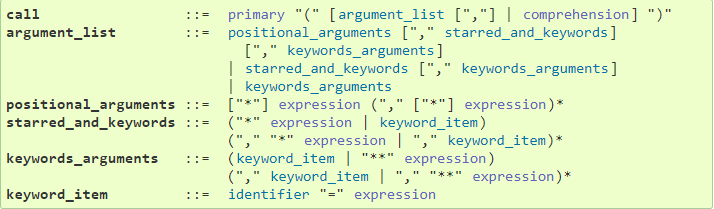
\includegraphics[scale=1]{call.jpg} 
可以在位置和关键字参数之后存在可选的尾随逗号,但不影响语义。\\
\indent primary必须计算可调用对象(用户定义的函数,内置函数,内置对象的方法,类对象,类实例的方法,以及具有__call __()方法的所有对象都是可调用的)。在尝试调用之前计算所有参数表达式。有关形式参数列表\href{https://docs.python.org/3/glossary.html#term-parameter}{parameter}的语法,请参阅\href{https://docs.python.org/3/reference/compound_stmts.html#function}{Function definitions}函数定义一节。\\
\indent 如果存在关键字参数,则首先将它们转换为位置参数,如下所示。首先,为形式参数创建未填充的slots列表。如果有N个位置参数,则将它们放在前N个slots中。接下来,对于每个关键字参数,标识符用于确定相应的slots(如果标识符与第一个形式参数名称相同,则使用第一个slots,依此类推)。如果slots已填充,则引发TypeError异常。否则,参数的值放在slots中,填充它(即使表达式为None,它填充slots)。处理完所有参数后,仍然未填充的slots将使用函数定义中的相应默认值填充。(默认值是在定义函数时计算的;因此,一个可变对象,例如用作默认值的列表或字典,将由未指定相应slots的参数值的所有调用共享;通常应该避免这种情况。)如果有任何未填充的slots没有指定默认值,则引发TypeError异常。否则,填充slot的列表将用作调用的参数列表。\\
\paragraph{CPython implementation detail:}内置函数可能提供了一些实现,其位置参数没有名称,即使它们为了文档的目的而“命名”,因此不能通过关键字提供。在CPython中,在C中实现的函数就是这种情况,它使用PyArg_ParseTuple()来解析它们的参数。\\
\indent 如果存在比正式参数slots更多的位置参数,则会引发TypeError异常,除非存在使用语法* identifier的形式参数;在这种情况下,该形式参数接收包含多余位置参数的元组(或者如果没有多余的位置参数则为空元组)。\\
\indent 如果任何关键字参数与形式参数名称不对应,则引发TypeError异常,除非存在使用语法**标识符的形式参数;在这种情况下,该形式参数接收包含多余关键字参数的字典(使用关键字作为键,参数值作为对应值),或者如果没有多余的关键字参数则接收(新)空字典。\\
\indent 如果语法*expression出现在函数调用中,则表达式必须求值为iterable。来自这些迭代的元素被视为它们是附加的位置参数。对于呼叫F(X1,X2,*Y,X3,X4),如果y的计算结果为一个序列Y1,... ,YM,这等同于用M + 4个位置参数X1,X2,Y1,...,y M的,x3,x4的调用。\\
\indent 这样做的结果是尽管*expression语法可能出现在显式关键字参数之后,但它在关键字参数(以及任何**expression参数 - 见下文)\textbf{之前}进行处理。所以:\\
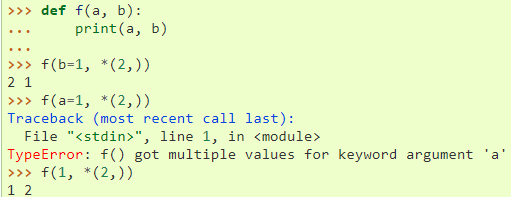
\includegraphics[scale=1]{arg.jpg} \\
\indent 在同一个调用中使用关键字参数和*expression语法是不常见的,因此在实践中不会出现这种混淆。\\
\indent 如果expression**表达式出现在函数调用中,则表达式必须求值为\textbf{映射},其内容被视为附加关键字参数。如果关键字已经存在(作为显式关键字参数,或来自另一个解包),则引发TypeError异常。\\
\indent 使用语法*identifier或**identifier的形式参数不能用作位置参数slots或关键字参数名称。\\
\indent 调用总是返回一些值,可能是None,除非它引发异常。如何计算此值取决于可调用对象的类型。它们是:\\
\begin{itemize}
\item a user-defined function:执行函数的代码块,并将参数列表传递给它。代码块首先要做的是将形式参数绑定到参数;这在功能定义一节中描述。当代码块执行return语句时,它指定函数调用的返回值。
\item a built-in function or method:结果取决于解释器;有关内置函数和方法的说明,请参阅内置函数。
\item a class object:A new instance of that class is returned.
\item a class instance method:调用相应的用户定义函数,其参数列表比调用的参数列表长一个:实例成为第一个参数。
\item a class instance:该类必须定义__call __()方法;效果就像调用该方法一样。
\end{itemize}

\section{Await表达式}
在一个awaitable的对象上暂停执行coroutine。只能在协同程序函数(coroutine function)中使用。\\
await_expr ::= "await" primary
\section{幂运算符}
幂运算符比左边的一元运算符绑定得更紧密;它比右边的一元运算符更紧密。语法是:\\
power ::=  (await_expr | primary) ["**" u_expr]\\
\indent 因此,在power和一元运算符的未表示序列中,运算符从右到左进行求值(这不会约束操作数的求值顺序): -1 ** 2得到-1。\\
\indent 当使用两个参数调用时,幂运算符具有与内置pow()函数相同的语义:它将其左参数提升为其右参数的幂。数字参数首先转换为公共类型,结果是该类型。\\
\indent 对于int操作数,结果与操作数具有相同的类型,除非第二个参数为负数;在这种情况下,所有参数都转换为float并传递float结果。例如,10 ** 2返回100,但10 ** - 2返回0.01。\\
\indent 将0.0增加到负幂会导致ZeroDivisionError。将负数增加到分数幂会导致数字复杂。 (在早期版本中它引发了一个ValueError。)
\section{一元算术和按位运算}
所有一元算术和按位运算具有相同的优先级:\\
u_expr ::= power | "-" u_expr | "+" u_expr | "~" u_expr \\
\indent 一元~(反转)运算符产生其整数参数的逐位反转。 x的按位求逆定义为 - (x + 1)。它仅适用于整数。
\section{二进制算术运算}
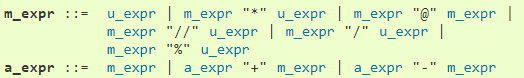
\includegraphics[scale=1]{binaryarithmetic.jpg} 
\indent *(乘法)运算符产生其参数的乘积。参数必须都是数字,或者一个参数必须是整数而另一个必须是序列。在前一种情况下,数字被转换为通用类型,然后相乘。在后一种情况下,\textbf{执行序列重复; 负重复因子产生空序列}。\\
\indent @(at)运算符旨在用于矩阵乘法。没有内置的Python类型实现此运算符。\\
\indent /(除法)和//(floor除法)运算符产生其参数的商。数字参数首先转换为通用类型。整数除法产生浮点数,而整数除法得到整数;结果是数学除法的结果,“floor”函数应用于结果。除以零会引发ZeroDivisionError异常。\\
\indent \%(modulo)运算符从第一个参数除以第二个参数得到余数。数字参数首先转换为通用类型。零右参数会引发ZeroDivisionError异常。参数可以是浮点数,例如,3.14\%0.7等于0.34(因为3.14等于4 * 0.7 + 0.34。)模运算符总是产生与第二个操作数(或零)具有相同符号的结果;结果的绝对值严格小于第二个操作数的绝对值。\\
\indent floor除法和模运算符通过以下标识连接:x ==(x // y)* y +(x\%y)。 Floor division和modulo也与内置函数divmod()连接:divmod(x,y)==(x // y,x\%y)。\\
\indent 除了对数字执行模运算之外,\%运算符还会被字符串对象重载以执行旧式字符串格式化(也称为插值interpolation)。字符串格式的语法在Python Library Reference,\href{https://docs.python.org/3/library/stdtypes.html#old-string-formatting}{printf-style String Formatting}部分中描述。\\
\indent floor除法运算符,模运算符和divmod()函数未定义复数。相反,如果合适,使用abs()函数转换为浮点数。\\
\indent +(加法)运算符产生其参数的总和。参数必须都是数字或两者都是相同类型的序列。在前一种情况下,数字被转换为通用类型,然后一起添加。在后一种情况下,序列是连接的。\\
\indent  -(减法)运算符产生其参数的差异。数字参数首先转换为通用类型。
\section{移位操作Shifting operaions}
移位操作的优先级低于算术操作:\\
\[shift_expr ::= a\_expr | shift\_expr ("<<" | ">>") a\_expr\]
\indent 这些运算符接受整数作为参数。它们将第一个参数向左或向右移动第二个参数给出的位数。右移n位被定义为由pow(2,n)进行的除法。左移n位被定义为与pow(2,n)的乘法。
\section{二进制按位运算}
$ \& \wedge \| $
\section{比较Comparsions}
与C不同,Python中的所有比较操作都具有相同的优先级,低于任何算术,移位或按位操作的优先级。与C不同,像$a <b <c$这样的表达式具有在数学中常规的解释:\\
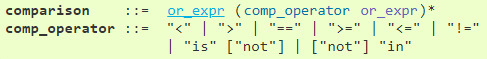
\includegraphics[scale=0.95]{comparsions.jpg} 
\indent 比较产生布尔值:True或False。
\indent 比较可以任意链接,例如,$x <y <= z$等于$x <y$和$y <= z$,除了y仅被评估一次(但在两种情况下,当$x <y$被发现时,根本不评估z是假的)。\\
\indent 形式上,如果a,b,c,...,y,z是表达式而op1,op2,...,opN是比较运算符,则op1 b op2 c ... y opN z等效于op1 b和b op2 c和... y opN z,除了每个表达式最多被计算一次。\\
\indent 注意,op1 b op2 c并不意味着a和c之间的任何比较,因此,例如$x <y> z$是完全合法的(尽管可能不是很漂亮)。
\subsection{值比较}
运算符$<, >, ==, > =. <=$和$!=$比较两个对象的值。对象不需要具有相同的类型。\\
\indent 章节对象,值和类型表明对象具有值(除了类型和标识)。对象的值在Python中是一个相当抽象的概念:例如,对象的值没有规范的访问方法。而且,不要求对象的值应以特定方式构造,例如,由其所有数据属性组成。比较运算符实现了对象值的特定概念。人们可以将它们视为通过比较实现间接定义对象的值。\\
\indent 因为所有类型都是(直接或间接)对象的子类型,所以它们从对象继承默认的比较行为。类型可以通过实现\href{https://docs.python.org/3/reference/datamodel.html#customization}{Basic customization}中描述的__lt__()等丰富的比较方法来自定义其比较行为。\\
\indent 相等性比较的默认行为(==和!=)基于对象的标识。因此,具有相同标志的实例的相等比较导致相等,并且具有不同标志的实例的相等性比较导致不等式。这种默认行为的动机是希望所有对象都应该是自反的(即x是y意味着$x == y$)。\\
\indent 未提供默认顺序比较($<,>,<=,> =$);尝试引发TypeError。这种默认行为的动机是缺乏与平等相似的不变量。\\
\indent 默认相等比较的行为,即具有不同标志的实例总是不相等的,可能与需要具有合理定义的对象值和基于值的相等性的类型形成对比。这些类型需要定制它们的比较行为,事实上,许多内置类型已经完成了。\\
\indent 以下列表描述了最重要的内置类型的比较行为。
\begin{itemize}
\item 内置数值类型(数字类型 - int,float,complex)和\\标准库类型fractions.Fraction和decimal.Decimal的数量可以在其类型内部和跨类型进行比较,但复数不支持顺序比较的限制。在所涉及类型的范围内,它们在数学上(算法上)正确地进行比较而不会损失精度。
\item 非数字值float('NaN')和decimal.Decimal('NaN')是特殊的。数字与非数字值的任何有序比较都是错误的。反直觉的含义是非数值不等于它们自身。例如,如果x = float('NaN'),则$3 <x, x <3, x == x, x != x$都是false。此行为符合IEEE 754。
\item 二进制序列(字节或bytearray的实例)可以在其类型内和跨类型进行比较。它们使用元素的数值按字典顺​​序进行比较。
\item 字符串(str的实例)使用字符的数字Unicode代码点(内置函数ord()的结果)按字典顺序进行比较。不能直接比较字符串和二进制序列。
\item 序列(元组,列表或范围的实例)只能在每种类型中进行比较,范围的限制不支持顺序比较。跨这些类型的相等比较会导致不等式,并且跨这些类型的排序比较会引发TypeError。\\
\indent 序列使用相应元素的比较按字典顺序进行比较,从而强制执行元素的反身性。\\
\indent 在强制元素的反身性时,集合的比较假定对于集合元素x,x == x总是为真。基于该假设,首先比较元素标识,并且仅针对不同元素执行元素比较。如果比较的元素是自反的,那么这种方法产生与严格元素比较相同的结果。对于非自反元素,结果与严格元素比较的结果不同,并且可能会令人惊讶:例如,非自反的非数字值在列表中使用时会产生以下比较行为:\\
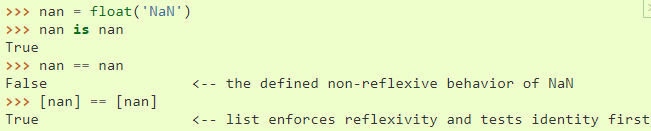
\includegraphics[scale=0.65]{compasions2.jpg} 
\end{itemize}

内置集合之间的字典比较如下:
\begin{itemize}
\item[1] 对于要比较的两个集合相等,它们必须是相同的类型,具有相同的长度,并且每对相应的元素必须比较相等(例如,[1,2] ==(1,2)是假的,因为类型不一样)。
\item[2] 支持顺序比较的集合的顺序与它们的第一个不等元素的比较啊顺序相同(例如,$[1,2,x] \leq [1,2,y]$与$x \leq y$具有相同的值)。如果不存在相应的元素,则首先排序较短的集合(例如,$[1,2] <[1,2,3]$为真)。
\end{itemize}
\indent 上接内置类型的比较行为。
\begin{itemize}
\item 当且仅当它们具有相等(key,value)对时,映射(dict的实例)才相等。键和值的相等比较强制实现反身性。\\
\indent 顺序比较($<, >, <=\textit{和}> =$)引发TypeError。
\item 集合(set或frozenset的实例)可以在其类型内和跨类型进行比较。\\
\indent 它们将顺序比较运算符定义为子集和超集测试。这些关系没有定义总排序(例如,两组集合{1,2}和{2,3}不相等,也不是彼此的子集,也不是彼此的超集。因此,对于依赖于总排序的函数,集合不是合适的参数(例如,min(),max()和sorted()在给定集合列表作为输入的情况下产生未定义的结果)。\\
\indent 集合的比较强制其元素的反身性。
\item 大多数其他内置类型没有实现比较方法,因此它们继承了默认的比较行为。
\end{itemize}
\indent 定制其比较行为的用户定义类应遵循一些一致性规则(如果可能):
\begin{itemize}
\item 平等比较应该是自反的。换句话说,相同的对象应该相等:x is y 意味着 x == y
\item 比较应该是对称的。换句话说,以下表达式应该具有相同的结果:x == y and y == x;x != y and y != x;$x < y$ and $y > x$;$x <= y$ and $y >= x$
\item 比较应该是可传递的。以下(非详尽的)示例说明:$x > y$ and $y > z$ 意味着 $x > z$;$x < y$ and $y <= z$ 意味着 $x < z$
\item 反向比较应该导致布尔否定。换句话说,以下表达式应该具有相同的结果:x == y and not x != y;$x < y$ and not $x >= y$ (for total ordering);$x > y$ and not $x <= y$ (for total ordering)\\
\indent 最后两个表达式适用于完全有序的集合(例如,序列,但不适用于集合或映射)。另请参见\href{https://docs.python.org/3/library/functools.html#functools.total_ordering}{total_ordering()}装饰器。
\item hash()结果应该具有平等一致性。相等的对象应具有相同的哈希值,或者标记为不可用。
\end{itemize}
\indent Python不强制执行这些一致性规则。实际上,非数字值是不遵循这些规则的示例。
\subsection{成员测试操作}
如果x是s的成员,则s in x计算结果为True,否则为False。 x not in s中返回s in x的否定。所有内置序列和集合类型都支持这个以及字典,在测试中字典是否具有给定键。对于容器类型,例如list,tuple,set,frozenset,dict或collections.deque,y in x表达式等于any(x is e or x == e for e in y)。\\
\indent 对于字符串和字节类型,当且仅当x是y的子字符串时,y中的x才为True。等效测试是y.find(x)!= -1。空字符串始终被视为任何其他字符串的子字符串,因此"" in "abc"将返回True。\\
\indent 对于定义\textbf{__contains__()}方法的用户定义类,如果y.__contains__(x)返回true值,则y in x返回True,否则返回False。\\
\indent 对于未定义__contains __()但定义__iter__()的用户定义类,如果在迭代y时产生一些x == z的值z,则y in x为True。如果在迭代期间引发异常,则就好像in引发异常一样。\\
\indent 最后,旧式迭代协议尝试:如果一个类定义了__getitem__(),则y in x为True,当且仅当存在非负整数索引i时,x == y[i],并且全部更低整数索引不会引发IndexError异常。 (如果引发任何其他异常,就好像in引发异常)。\\
\indent not in运算符被定义为具有in的反向真值
\subsection{身份比较}
运算符is和is not对象标识的测试:当且仅当x和y是同一个对象时,x is y为真。使用id()函数确定对象标识。 x is not y产生反向真值。

\section{布尔运算}
在布尔运算的上下文中,以及控制流语句使用表达式时,以下值被解释为false:False,None,所有类型的数字零,以及空字符串和容器(包括字符串,元组,列表,字典) ,集合和frozensets)。\\
\indent 如果运算符的参数为false,则运算符not返回True,否则返回False。\\
\indent 表达式x和y首先计算x;如果x为false,则返回其值;否则,将计算y并返回结果值。\\
\indent 表达式x或y首先评估x;如果x为真,则返回其值;否则,将计算y并返回结果值。\\
\indent 请注意,它们既不返回也不限制它们返回False和True的值和类型,而是返回最后一个求值的参数。这有时是有用的,例如,如果s是一个字符串,如果它是空的,则应该用默认值替换,表达式s or 'foo'产生所需的值。因为not必创建新值,所以无论其参数的类型如何,它都会返回一个布尔值(例如,not 'foo'会生成False而不是''。)

\section{条件表达式}
条件表达式(有时称为“三元运算符”)具有所有Python操作的最低优先级。\\
\indent 表达式x if C else y首先计算条件,C而不是x。如果C为真,则计算x并返回其值;否则,计算y并返回其值。\\
\indent 有关条件表达式的更多详细信息,请参阅\href{https://www.python.org/dev/peps/pep-0308}{PEP 308}。
\section{Lambdas表达式}
lambda_expr ::= "lambda" [parameter_list] ":" expression \\
\indent lambda_expr_nocond ::= "lambda" [parameter_list] ":" expression_nocond\\
\indent Lambda表达式(有时称为lambda表单)用于\textbf{创建匿名函数}。表达式lambda parameters: expression产生一个函数对象。未命名的对象的行为类似于使用以下定义的函数对象:\\
def <lambda>(parameters):return expression\\
\indent 有关参数列表的语法,请参阅\href{https://docs.python.org/3/reference/compound_stmts.html#function}{Function definitions}一节。请注意,使用lambda表达式创建的函数不能包含语句或注释。
\section{表达式列表}
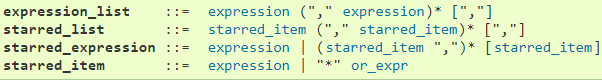
\includegraphics[scale=0.8]{expressionlist.PNG}\\
\indent 除非列表或集合显示的一部分,否则包含至少一个逗号的表达式列表会产生元组。\\
\indent 星号$\star$表示可迭代的解包(\textit{iterable unpacking})。它的操作数必须是可迭代的。迭代被扩展为一系列条目,这些条目包含在解包的新元组,列表或集合中。\\
\indent \textit{版本3.5中的新功能}:表达式列表中的可迭代解包,最初由PEP 448提出。\\
\indent 尾随逗号只需要创建一个元组(a.k.a. \textit{a singleton});在所有其他情况下它是可选的。没有尾随逗号的单个表达式不会创建元组,而是生成该表达式的值。 (要创建一个空元组,请使用一对空括号:()。)
\section{计算顺序}
Python从左到右计算表达式。请注意,在计算赋值时,右侧在左侧之前进行计算。\\
\indent 在以下行中,表达式将按其后缀的算术顺序进行计算:\\
\begin{itemize}
\item expr1, expr2, expr3, expr4
\item (expr1, expr2, expr3, expr4)
\item {expr1: expr2, expr3: expr4}
\item expr1 + expr2 * (expr3 - expr4)
\item expr1(expr2, expr3, *expr4, **expr5)
\item expr3, expr4 = expr1, expr2
\end{itemize}
\section{运算符优先级}
下表总结了Python中的运算符优先级,从最低优先级(最小绑定)到最高优先级(大多数绑定)。同一个框中的运算符具有相同的优先级。除非明确给出语法,否则运算符是二进制的。同一个框组中的操作符从左到右(取幂除外,从右到左分组)。\\
\indent 请注意,比较,成员测试和身份测试都具有相同的优先级,并具有从\href{https://docs.python.org/3/reference/expressions.html#comparisons}{Comparisons}部分中所述的从左到右的链接功能。\\
\includegraphics[scale=0.8]{operatorprecedence.PNG} 
\end{document}